\section{What is OpenGL?}
\label{sec:opengl}
OpenGL is an open source graphics library providing an application programming interface (API) to communicate with a graphics processing unit (GPU) in order to get hardware-accelerated \textit{rendering}. Rendering is the process of generating an image from \textit{models} in an \textit{environment}. These models contain information about the geometry and associated textures. A model is typically represented by a set of points, triangles or some other set of \textit{primitives}. Before discussing the model and the environment, we should explain what a primitive is.
\subsection{Primitive}
In OpenGL, the primitive decides how to interpret a set of vertices. The same set of vertices may be interpreted, hence rendered, very different on the screen. Three points can be used to draw three single points, a triangle or a part of a rectangle among other different geometries. To illustrate this idea, in figure \ref{fig:opengl_primitives}, the four vertices $\{(0,0), (0,1), (1,1), (1,0)\}$ have been rendered with the primitives \textit{GL\_POINTS}, \textit{GL\_LINES}, \textit{GL\_TRIANGLES}, \textit{GL\_QUADS} and \textit{GL\_TRIANGLE\_STRIP}. The rendered objects are of course very different depending on the primitive. 
\begin{figure}[h]
\begin{center}

\includegraphics[width=\textwidth, trim=0cm 0cm 0cm 0cm, clip]{opengl/figures/primitives.png}
\end{center}
\caption{The vertices $\{(0,0), (0,1), (1,1), (1,0)\}$ have been rendered as the primitives (from left) \textit{GL\_POINTS}, \textit{GL\_LINES}, \textit{GL\_TRIANGLES}, \textit{GL\_QUADS} and \textit{GL\_TRIANGLE\_STRIP}. We see that the final rendered geometrical objects are quite different for the different primitives.}
\label{fig:opengl_primitives}
\end{figure}
When using for example the \textit{GL\_TRIANGLES}, OpenGL interprets groups of three vertices as one triangle. In the case of \textit{GL\_QUADS}, it will of course use groups of four vertices to define the renderable object. All of the primitives (except the \textit{GL\_POINTS}) form one or more two dimensional surfaces that are colored from either the interpolated values between the vertices or from a texture map which we now will explain.
\subsection{Color interpolation}
\label{sec:opengl_color_interpolation}
When creating a primitive consisting of $N$ vertices we can color each vertex $\vec r_i$ with an RGBA vector
\begin{align}
	\vec c_i = (r_i, g_i, b_i, \alpha_i)
\end{align}
where the components are the red, green, blue and alpha values for vertex $i$. The first three components defines the color whereas the last component is the transparency. In between the $N$ vertices, there are a lot of points that do not have a defined color value. OpenGL assigns colors to these inner points by \textit{linearly interpolating} the color values of the vertices. Any point $\vec p$ in a triangle defined by the three vertices $\vec p_a, \vec p_b$ and $\vec p_c$ can be uniquely specified by using \textit{barycentric coordinates} which is a set of three numbers $(a,b,c)$ in the range $[0,1]$, normalized so that $a+b+c=1$. \todo{cite the opengl specification} Once we have these coordinates, the point $\vec p$ in the global coordinate system (in which the vertices $\vec p_i$ are defined) is found as
\begin{align}
	\vec p = a\vec p_a + b\vec p_b + c\vec p_c.
\end{align}
The barycentric coordinates are found through
\begin{align}
	a = \frac{A(\vec p, \vec p_b, \vec p_c)}{A(\vec p_a, \vec p_b, \vec p_c)}, \qquad b = \frac{A(\vec p, \vec p_a, \vec p_c)}{A(\vec p_a, \vec p_b, \vec p_c)}, \qquad c = \frac{A(\vec p, \vec p_a, \vec p_b)}{A(\vec p_a, \vec p_b, \vec p_c)}.
\end{align}
We then use the barycentric coordinates as the weights in the linear interpolation so that the color at a point $\vec p$ is given as
\begin{align}
	\vec c(\vec p) = a\vec c_a + b\vec c_b + c\vec c_c,
\end{align}
where $\vec c(\vec p_i)$ is the color we gave the vertex at $\vec p_i$. In figure \ref{fig:opengl_color_interpolation} we see how the colors are interpolated from the three values at the triangle vertices.
\begin{figure}[h]
\begin{center}
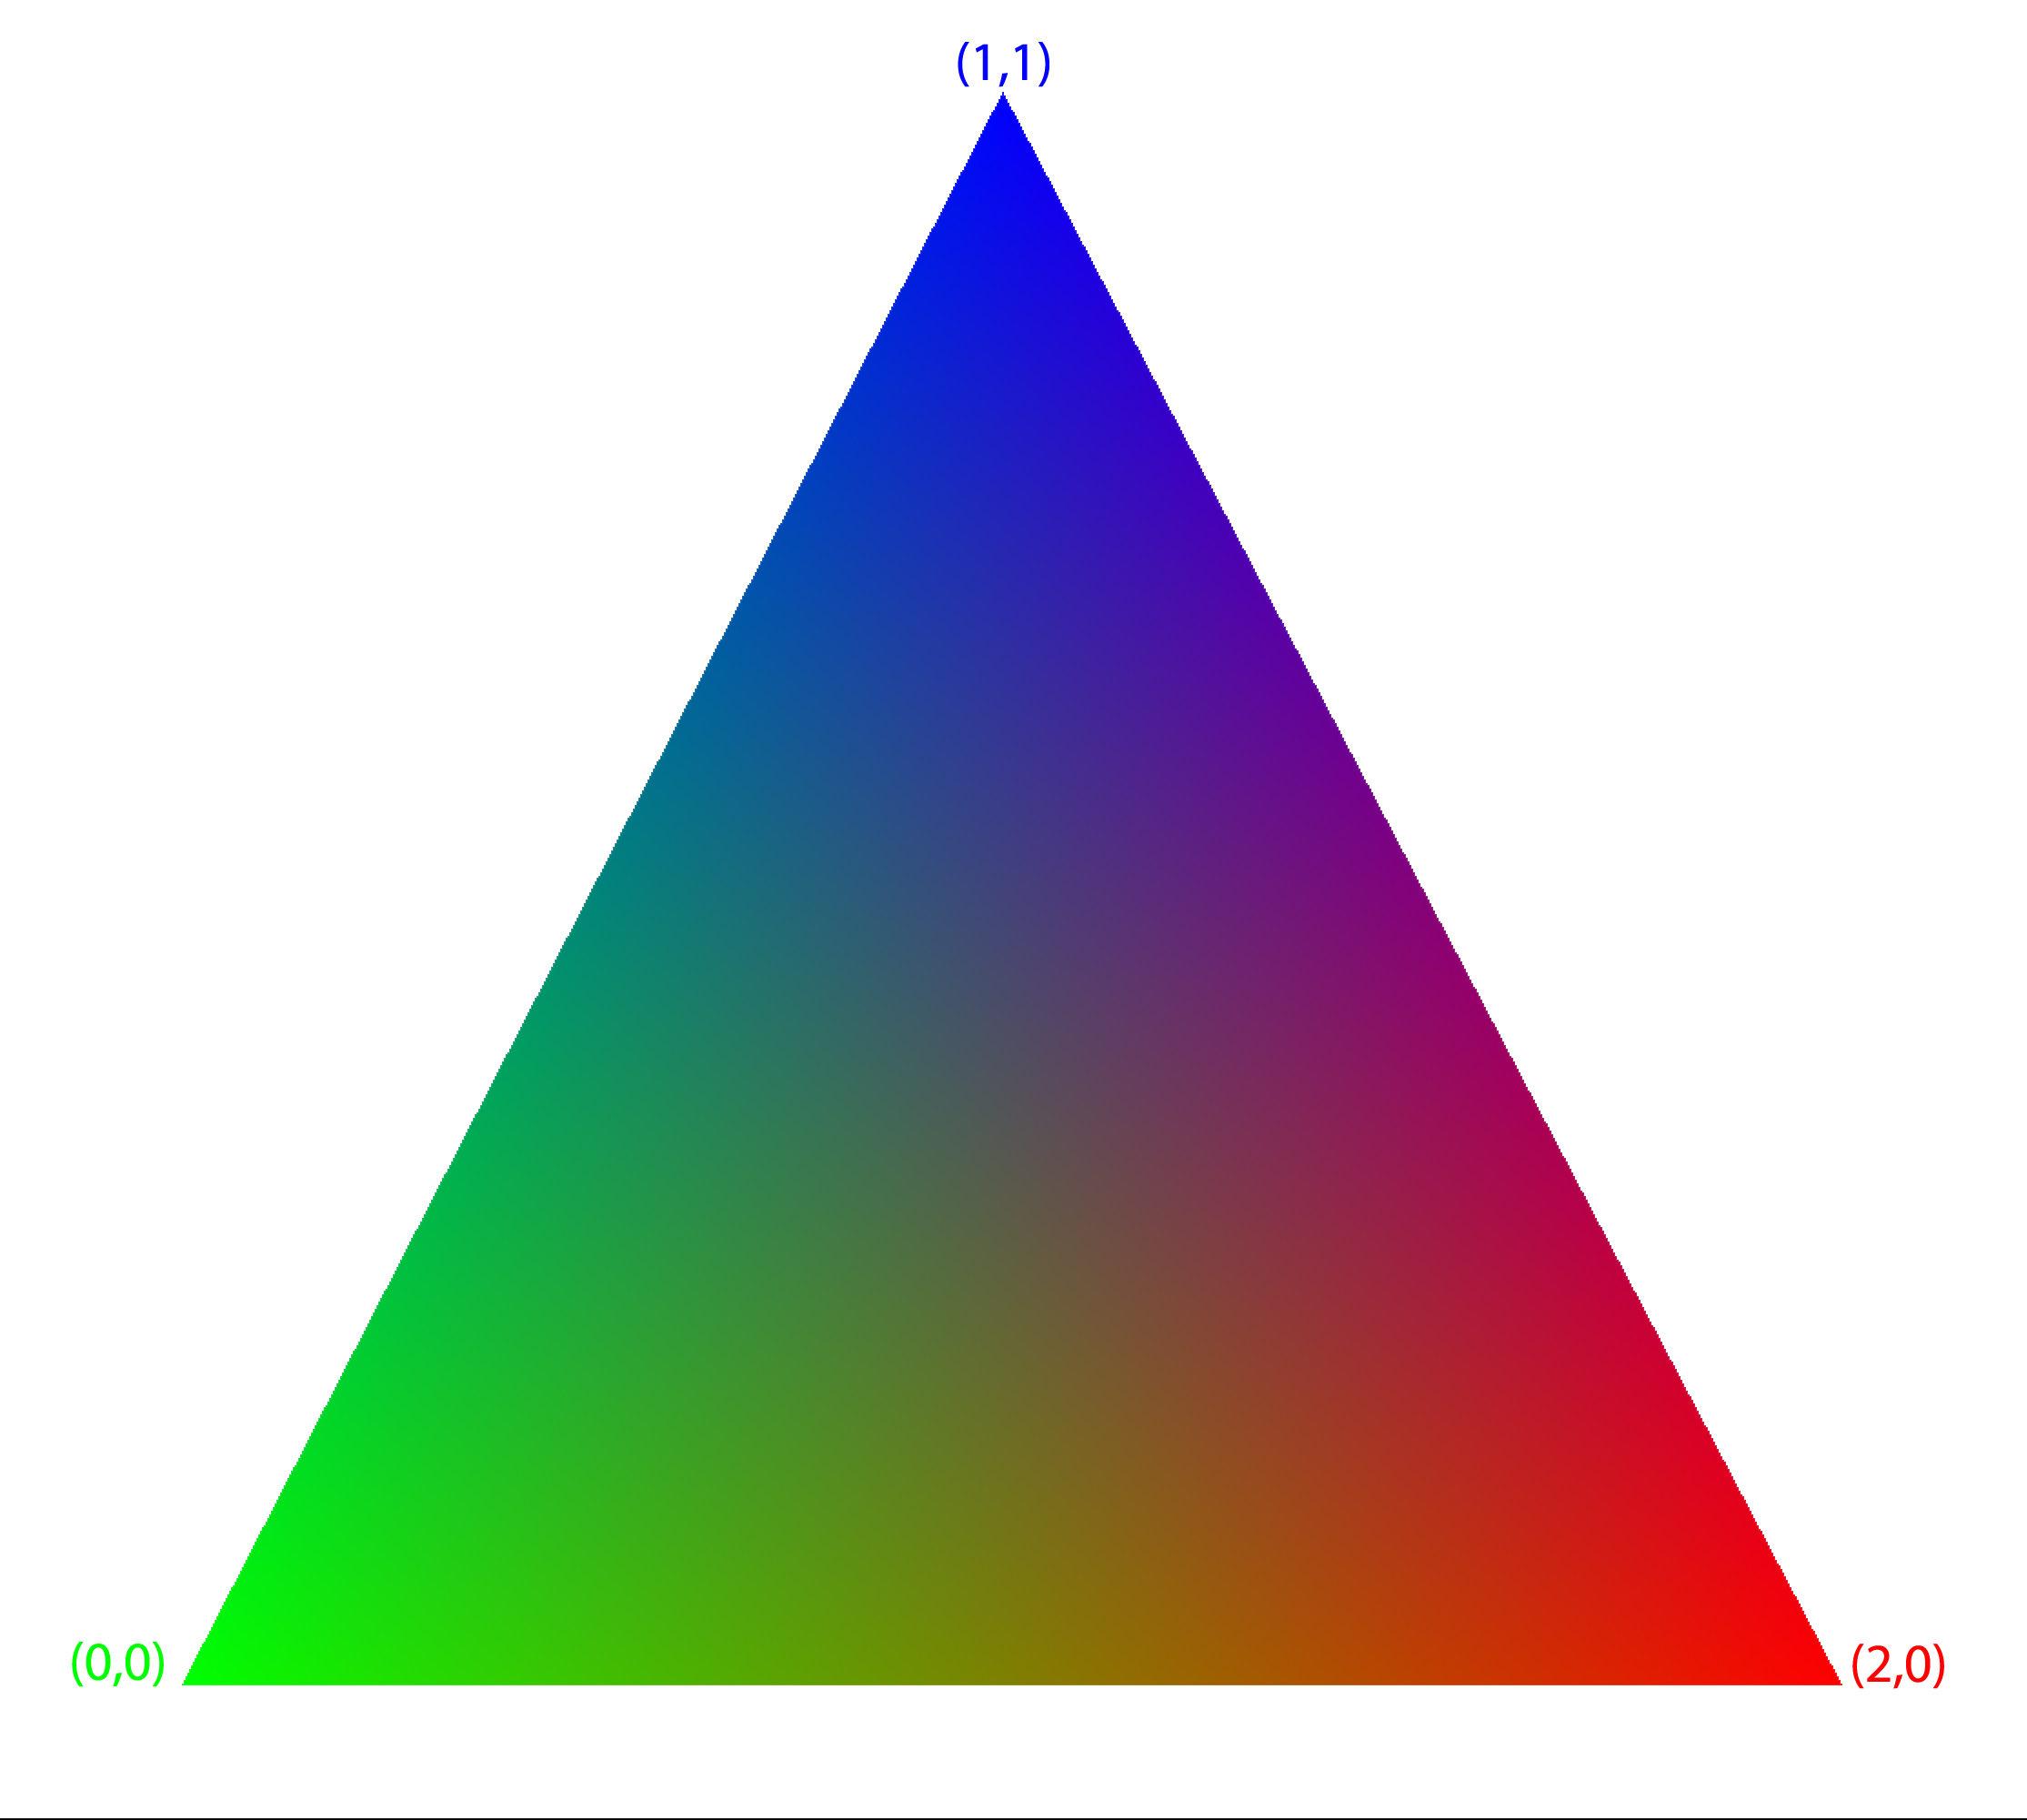
\includegraphics[width=\textwidth, trim=0cm 0cm 0cm 0cm, clip]{opengl/figures/color_interpolation.png}
\end{center}
\caption{The three vertices $\{(0,0), (1,1), (2,0)\}$ colored green, blue and red, forms a triangle where the inner points of the triangle is colored by the interpolation between the three vertices.}
\label{fig:opengl_color_interpolation}
\end{figure}
\subsection{Textures}
\label{sec:opengl_texture_interpolation}
Instead of using the colors specified per vertex, we can upload a texture (for example an image) to the graphics card so that the GPU can use that as the source of the color (this can be combined with the color values as we will see soon). The texture consists of $m\times n$ pixels where each pixel has a color $\vec c_t$. Each vertex $i$ of the triangle is assigned a \textit{local texture coordinate} 
\begin{align}
	\vec t_i = (t_x, t_y),
\end{align}
where $t_x, t_y \in [0,1]$. This gives the mapping to the \textit{global texture coordinates} (the actual pixel coordinates) $\vec t^* = (t_x^*, t_y^*)$ where 
\begin{align}
	\nonumber
	t_x^* &= m\cdot t_x\\
	t_y^* &= n\cdot t_y,
\end{align}
where we have added the asterisk on the global coordinates since we will mostly use the local ones. Since each pixel $\vec t$ (remember these are the local coordinates) in the texture has a color value $\vec c_t(\vec t)$, we can find the color $\vec c(\vec p)$ of a point $\vec p$ within the triangle by interpolating the local texture coordinates as we interpolated the colors. Remember that the point $\vec p$ has barycentric coordinates $(a,b,c)$, so the local texture coordinates $\vec t$ are found by
\begin{align}
	\vec t(\vec p) =  a\vec t_a + b\vec t_b + c\vec t_c,
\end{align}
where $\vec t_i$ is the local texture coordinate assigned to vertex $i$. The color of this point $\vec p$ is then simply
\begin{align}
	\vec c(\vec p) = \vec c_t[\vec t(\vec p)].
\end{align}
In figure \ref{fig:opengl_texture_interpolation} we have illustrated how the texture interpolation works. In the left figure, the texture is mapped with  texture coordinates corresponding to the coordinates of the triangle vertices. In the figure to the right we have a skewed mapping making the image look skewed.
\begin{figure}[h]
\begin{center}
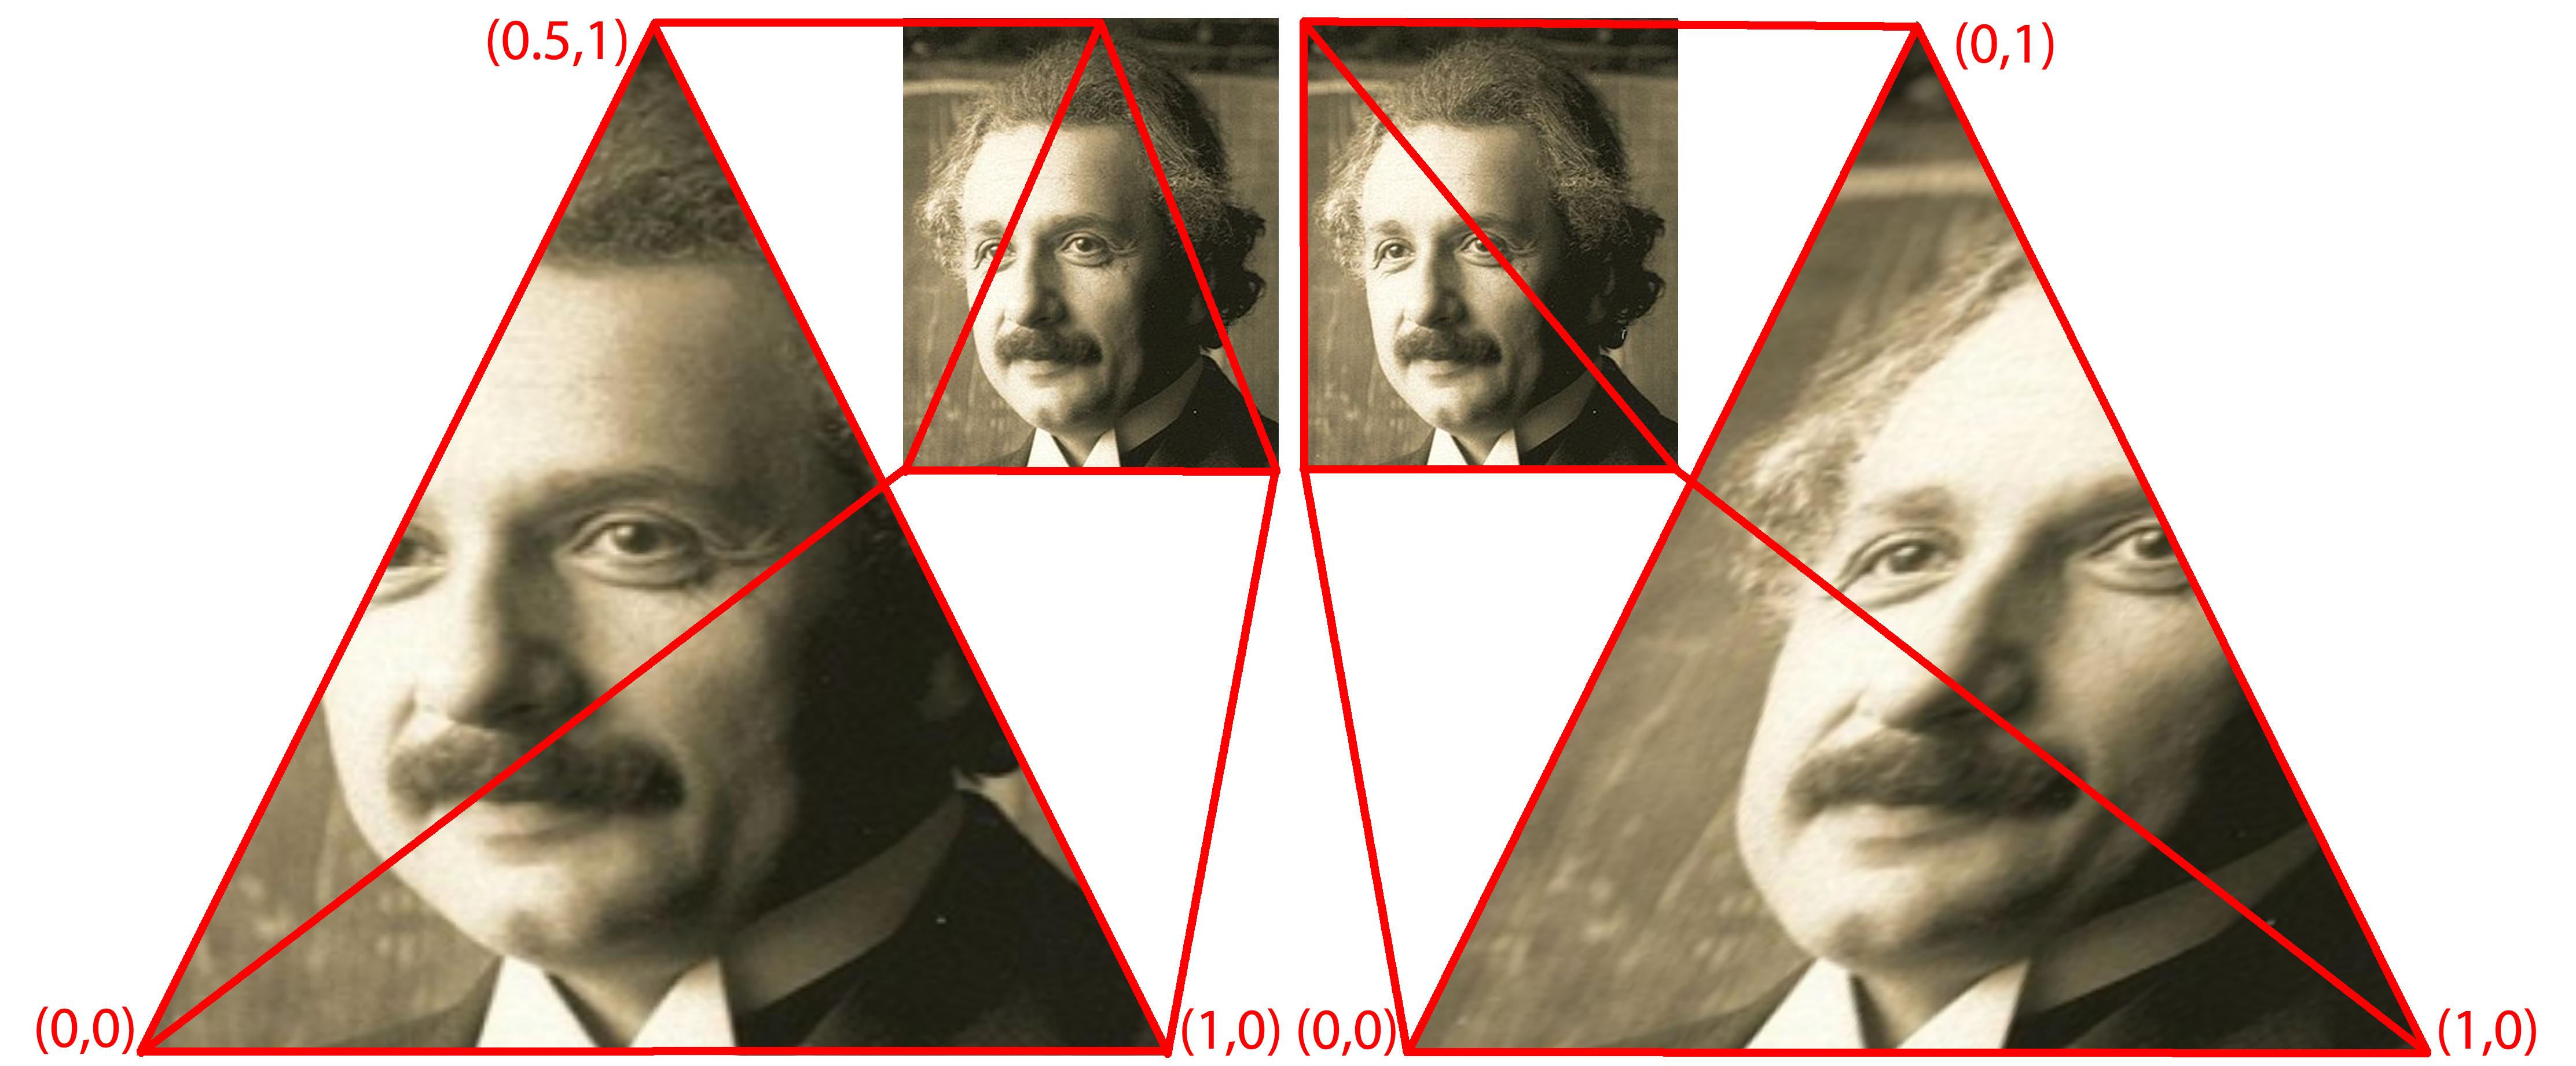
\includegraphics[width=\textwidth, trim=0cm 0cm 0cm 0cm, clip]{opengl/figures/texture_interpolation.png}
\end{center}
\caption{Showing how texture interpolation works. Left: the three vertices $\{(0,0), (1,1), (2,0)\}$ are assigned the local texture coordinates $\{(0,0), (0.5,1), (1,0)\}$ where we see how the texture are transformed onto the triangle . Right: the three vertices $\{(0,0), (1,1), (2,0)\}$ are assigned the local texture coordinates $\{(0,0), (0,1), (1,0)\}$ where we see that the texture on the triangle is skewed because of the transformation. Note that the coordinates in the figure at the vertices are the texture coordinates, not the coordinates of the vertices.}
\label{fig:opengl_texture_interpolation}
\end{figure}
We can of course combine both these methods (colors and textures) by applying both a texture coordinate \textit{and} a color value to each vertex. OpenGL will then render an image where the rendered color $\vec C$ becomes
\begin{align}
	\label{eq:opengl_combining_colors_textures}
	\vec C(\vec p) = \vec c_t[\vec t(\vec p)] \odot \vec c(\vec p),
\end{align}
where $\odot$ is the element-wise multiplication operator defined as
\begin{align}
	(\vec a \odot \vec b)_i = a_i\cdot b_i,
\end{align}
where $\vec a,\vec b \in \mathbb{R}^N$ and $d_i$ is the $i$'th component of $\vec d$. In figure \ref{fig:color_and_texture} we have combined both the color and the texture giving a triangle with the same image of Albert Einstein colored as in figure \ref{fig:opengl_color_interpolation}.
\begin{figure}[h]
\begin{center}

\includegraphics[width=\textwidth, trim=0cm 0cm 0cm 0cm, clip]{opengl/figures/color_and_texture.png}
\end{center}
\caption{We can combine both colors and textures to color points within a triangle according to equation \eqref{eq:opengl_combining_colors_textures}. Here we have used the same colors as in figure \ref{fig:opengl_color_interpolation} and the texture of Albert Einstein in figure \ref{fig:opengl_texture_interpolation}.}
\label{fig:color_and_texture}
\end{figure}
\subsection{Model}
\label{sec:opengl_model}
A model of an object contains all the information fully defining how a geometric object looks like without any effects from the environment such as light or distortions from a water surface. The model is fully described by a set $\mathcal{M}$ containing primitive objects $\mathcal{P}$, each having 
\begin{itemize}
	\item a vertex array,
	\item the primitive type,
	\item a color array,
	\item a texture id,
	\item a local texture coordinate array, and
	\item a normal vector array.
\end{itemize}
We have discussed the array of vertices, the primitive, the color and texture coordinate arrays (remember, one color and/or one texture coordinate per vertex). We also need the id (which is just an int variable) allowing us to tell the GPU which texture it should apply to this primitive object. In addition, we can assign a \textit{normal vector} to each vertex which can be used to create realistic lighting and other effects. It's time for an example of a model.\\
Say we want a model of a die. A die is a cube with six faces. The model $\mathcal M$ would then contain six primitive objects $\mathcal P_i$, each having an array of four vertices. The primitive type would be \textit{GL\_QUADS} where the color of course could be your favorite. We need to upload six textures (one face has one dot, another face has two dots etc) which gives us six different texture id's. The local texture coordinate array is simply the four corners of the unit square whereas the normal vectors should point outwards from the cube. In figure \ref{fig:opengl_die} we haved used this technique to draw a red die.
\begin{figure}[h]
\begin{center}
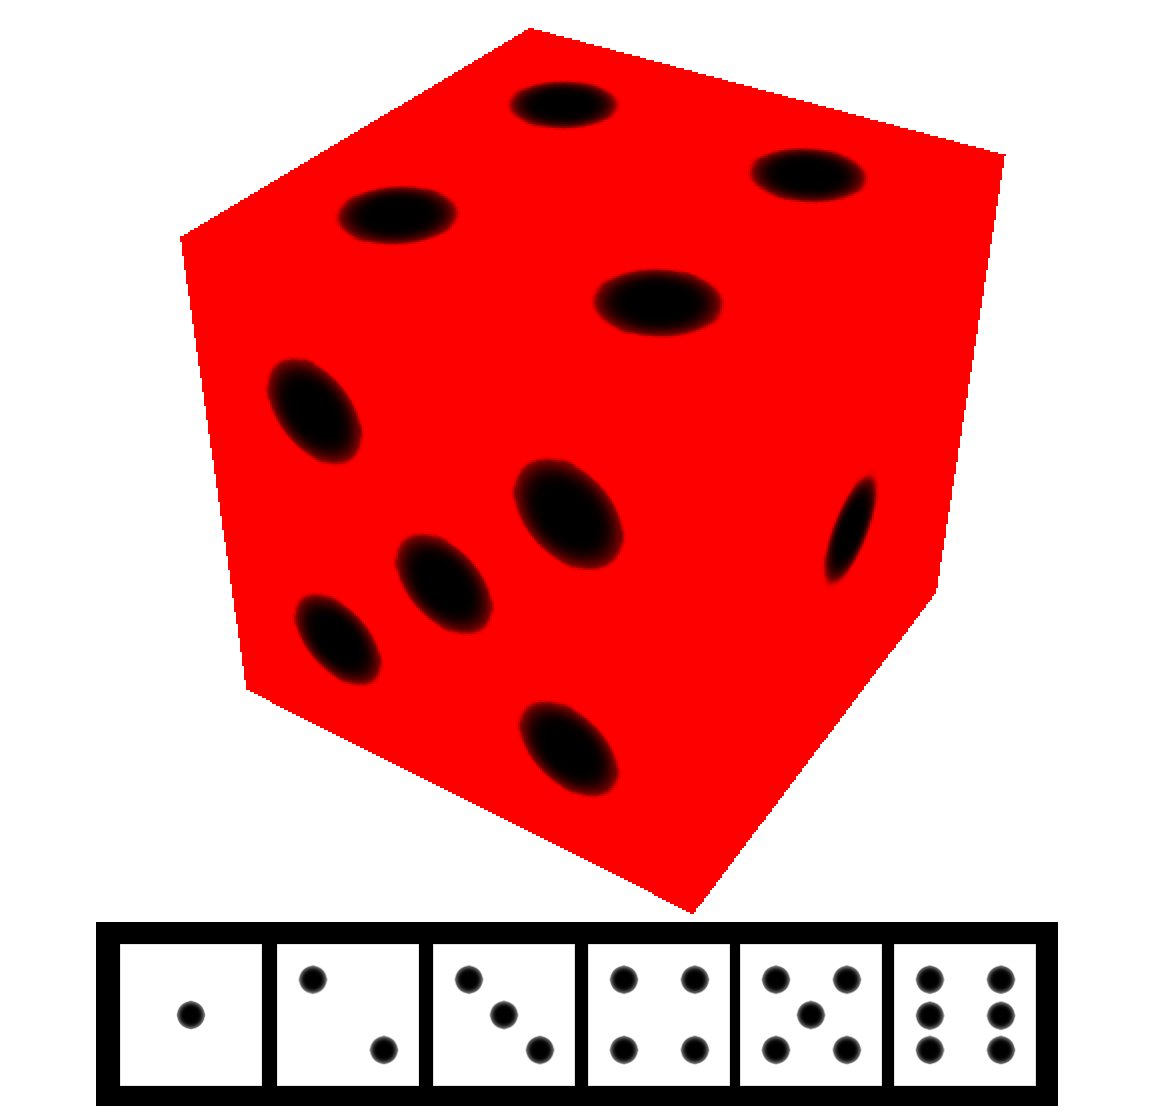
\includegraphics[width=\textwidth, trim=0cm 0cm 0cm 0cm, clip]{opengl/figures/die.png}
\end{center}
\caption{Drawing a die using the technique described in subsection \ref{sec:opengl_model}. The color was chosen to be red whereas each of the six faces were assigned one of the textures in the black box.}
\label{fig:opengl_die}
\end{figure}
\subsection{Environment}
